
\documentclass{beamer}
\usepackage[utf8]{inputenc}
\usetheme{Dresden}
\usecolortheme{beaver}
\setbeamercolor{itemize item}{fg=darkred!80!black}
\usepackage[ruled, czech, linesnumbered, noline, longend]{algorithm2e}
\usepackage{times}
\usepackage{multirow}
\usepackage{graphics}
\usepackage{pdflscape}
\usepackage{hyperref}
\usepackage[czech]{babel}
\usepackage{listings}

\title{Typografie a publikování - 5. projekt}
\subtitle{Bublinkové řazení}
\author{Jiří Štípek}
\institute
{
	Vysoké učení technické v~Brně\\
	Fakulta informačních technologií
}
\date{\today}

\begin{document}
\frame{\titlepage}
\begin{frame}{Obsah}
    \setbeamertemplate{section in toc}[sections numbered]
    \tableofcontents[hideallsubsections]
\end{frame}
\section{Co to vlastně bublinkové řazení je?}
\begin{frame}{Co to vlastně bublinkové řazení je?}
\begin{itemize}
    \item Bublinkové řazení (známé pod anglickým jménem bubble sort, česky též řazení záměnou) je implementačně jednoduchý řadicí algoritmus
\end{itemize}
    
\end{frame}
\section{Princip}
\begin{frame}{Princip}
    \begin{itemize}
        \item porovnává postupně v celém poli dva sousední prvky; pokud nejsou ve správném pořadí, zamění je
        \item po tomto kroku je na posledním místě pole největší prvek (\uv{probublá} na konec)
        \item krok algoritmu probublávání aplikuje postupně na zbytek pole o délce n-1, n-2,…,2
       
    \end{itemize}
\end{frame}
\section{Barevný diagram bublinkového řazení}
\begin{frame}{Barevný diagram bublinkového řazení}
\begin{center}
    \scalebox{0.17}
    {
    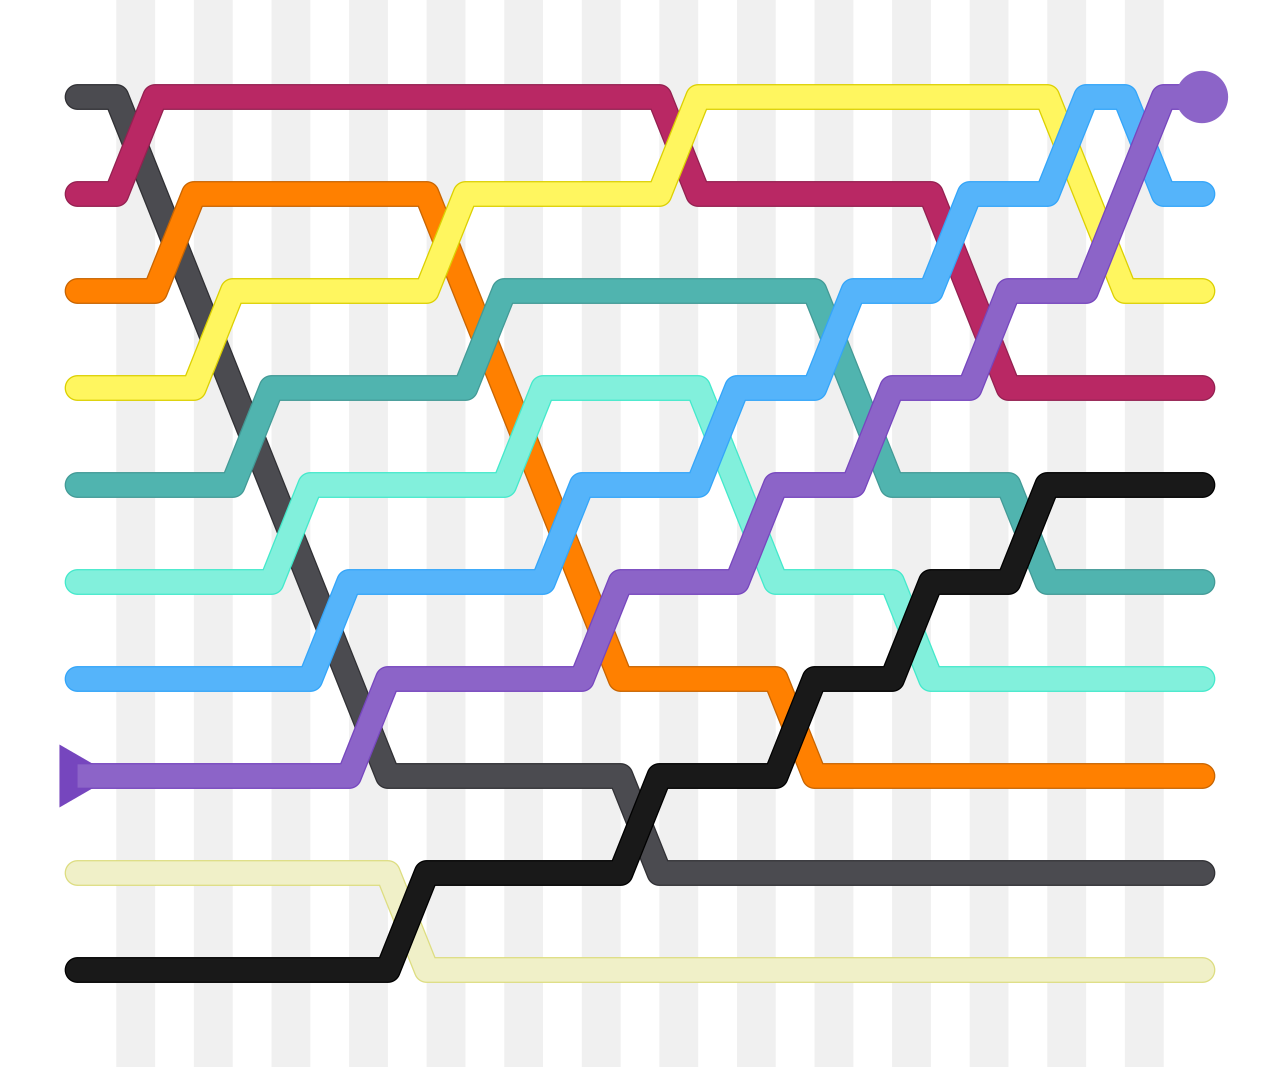
\includegraphics{Bubliny.png}
    }
\end{center}
\end{frame}
\section{Pseudokód}
\begin{frame}{Pseudokód}
    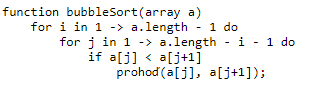
\includegraphics{pseudokod.png}
\end{frame}
\section{Výhody}
\begin{frame}{Výhody bublinkového řazení}
    \begin{itemize}
        \item nejjednodušší na naprogramování
        \item stabilní, tzn. nemění pozici prvků, které jsou při porovnávání vyhodnoceny jako ekvivalentní
        \item algoritmus nepotřebuje v řazené posloupnosti provádět žádné skoky
    \end{itemize}
\end{frame}
\section{Nevýhody}
\begin{frame}{Nevýhody bublinkového řazení}
    \begin{itemize}
        \item pro řazení opravdu velkých polí je bublinkové řazení naprosto nevhodné
        \item zbytečná porovnání při řazení seznamu s nejnižším prvkem na konci
    \end{itemize}
\end{frame}
\begin{frame}
\begin{center}
    \Large{Děkuji za pozornost !}
\end{center}
\end{frame}
\begin{frame}{Zdroje}
    https://www.fd.cvut.cz/personal/xfabera/14PRG/cviceni9/razeni.pdf\\
    https://en.wikipedia.org/wiki/BubbleSort\\
    https://www.algoritmy.net/article/3/Bubble-sort\\
\end{frame}
\end{document}
